\documentclass[11pt]{article}
\usepackage[T1]{fontenc}
\usepackage{hyperref}
\hypersetup{
    colorlinks=true,
    linkcolor=blue,
    filecolor=magenta,      
    urlcolor=blue,
    pdftitle={Pion Scattering},
    pdfpagemode=FullScreen,
    }
\usepackage[margin=1in]{geometry}
\usepackage{amsmath}
\usepackage[parfill]{parskip}
\usepackage{bigints}
\usepackage{tikz}
\usepackage{titling}
\usepackage{listings}
\usepackage{bbm}
\setlength{\droptitle}{-10em}  
\newcommand{\bv}{\boldsymbol}
\newcommand{\br}[1]{\left\langle #1 \right |}
\newcommand{\kt}[1]{\left| #1 \right \rangle}
\newcommand{\bkt}[2]{\left \langle #1 |#2 \right \rangle}
\newcommand{\brkt}[3]{\left\langle #1 \right |#2 \left| #3 \right \rangle}
\newcommand\ddfrac[2]{\frac{\displaystyle #1}{\displaystyle #2}}
\newcommand{\note}[1]{\color{red} #1 \color{black}}
\newcommand\mo{\mathcal{O}}
\newcommand\mm{\mathcal{M}}
\newcommand{\e}{\mathrm{e}}
\newcommand{\ot}{_{12}}
\newcommand{\tot}{t_{12}}
\newcommand{\totp}{t'_{12}}
\newcommand{\mpi}{m_\pi}
\newcommand{\mn}{m_{{}_N}}
\newcommand{\sq}{^{\,2}}
\author{Alexander P Long}
\title{Elastic Pion Scattering Kernel Derivation}

\begin{document}
%Diagrams made and can be edited with https://www.mathcha.io/editor under alexlong@gwmail.gwu.edu email account
\maketitle
This follows the conventions from the \href{https://arxiv.org/abs/hep-ph/9501384v1}{BKM (Bernard, Kaiser, Meissner)  review}, including the use of $F_\pi=93.1$, see table 2 on page 23 of the review, however it is not clear if $F$ in the appendix, differs from $F_\pi$, by a factor of $\pi$. If this is the case a lot of things would make more sense.
The BKM review also goes over this reaction on pg 115 for the two body case.\\

There are a few sources for pion scattering at zero energy:\\
\href{https://arxiv.org/abs/hep-ph/0206219v1}{S-wave scattering length: Beane 2002}\\~\\
\href{https://www.sciencedirect.com/science/article/abs/pii/037026939290099P}{Weinberg 1992}, includes isospin dependence. \href{https://arxiv.org/pdf/hep-ph/9209257.pdf}{ArXiV link} doesn't have diagrams.
Note Weinberg uses $F_\pi=186 \mathrm{MeV}$, so converting to the BKM convention requires a factor of 2.
% In the Weinberg paper he states that the pion propagator is $ \left( \vec{q}^2 +m_\pi^2 \right)^{-1} $ but where does this come from? Why isn't it just $ \left( q^2 -m_\pi^2 + i \varepsilon \right)^{-1}  $ like it says in the NuPa cheat sheet.
\tableofcontents
\section{Identities, Definitions, and Useful Identities}
\begin{equation}
    \sigma_j \sigma_k = \delta_{jk} I + i \varepsilon_{jk\ell} \sigma_{\ell}
\end{equation}
\begin{equation}
    \mu= \frac{m_\pi}{m_{nucl}}
\end{equation}
\begin{equation}
    F_\pi=93.1 \mathrm{MeV}
\end{equation}
For our purposes the incoming and outgoing pions have the same charges.

Notation with momentum four vectors can be confusing, so in this document, for $4$-vectors $p$ and $q$, use the notation
$p-q$ to represent:
\begin{align}
    p-q&= (\sqrt{m_p+\vec{p}\sq}, \vec{p}) + (\sqrt{m_q+\vec{q}\sq},-\vec{q})\\
       &= \left(\sqrt{m_p+\vec{p}\sq}+\sqrt{m_q+\vec{q}\sq},\vec{p}-\vec{q} \right)\\
       &= \left(p_0+q_0,\vec{p}-\vec{q} \right)
\end{align}
I'm ~pretty sure~ this make sense to do, but I'm completely set on it. Additionally this means, that unless otherwise
stated:
\begin{equation}
    -p= \left( \sqrt{m_p^2 + \vec{p}\sq },-\vec{p} \right)
\end{equation}
\subsubsection{Prefactor}
I'm pretty sure that each diagram comes with a prefactor of:
\begin{equation}
    \frac{1}{2 \left( 1+\mu \right) }\quad\text{or}\quad \frac{1}{2 \left( 1+\mu \right) \pi^4}
\end{equation}
\subsubsection{Definition of the spin vector}
There is still some confusion on the definition of the zeroth element of $S$.

\href{https://en.wikipedia.org/wiki/Relativistic_angular_momentum#Spin_in_special_relativity}{This source}
implies its zero up to relativistic corrections. Consider the rest frame, and boosted (lab frame) spins:
\begin{equation}
    \text{Rest frame:}\quad S'= (0, s_x',s_y',s_z')
    \qquad\text{Lab frame:}\;
    S=(s_t, s_x,s_y,s_z)
\end{equation}
This must be Lorentz invariant, so 
\begin{equation}
    s_t^2 - \vec{s}\cdot \vec{s} = - \vec{s}\,' \cdot \vec{s}\,'
\end{equation}
Its easier to calculate the rest frame in terms of a boost on the lab frame, so:
\begin{align}
{S'}^{0}&={\Lambda ^{0}}_{\alpha }S^{\alpha }={\Lambda ^{0}}_{0}S^{0}+{\Lambda ^{0}}_{i}S^{i}=\gamma \left(S^{0}-U_{i}S^{i}\right)\\
        &=\gamma \left(S^{0}-u_i S^{i}\right)=U_{0}S^{0}-U_{i}S^{i}\\
        &=U_\alpha S^\alpha=0\quad\text{(invariant)}\\
        &\nonumber\\
{S'}^{i}&={\Lambda ^{i}}_{\alpha }S^{\alpha }={\Lambda ^{i}}_{0}S^{0}+{\Lambda ^{i}}_{j}S^{j}\\
        &=-\gamma U^{i}S^{0}+\left[\delta _{ij}+{\frac {\gamma -1}{\vec{U}^{\,2}}}U_{i}U_{j}\right]S^{j}\\
        & =S^{i}+{\frac {\gamma ^{2}}{\gamma +1}}U_{i}U_{j}S^{j}-\gamma U^{i}S^{0}
\end{align}
Note that $S'^0=0$ 
Note $U_\alpha S^\alpha=0$\\
Where $U$ is the 3-velocity that boosts the particle to the lab frame. Inverting the above gives the spin in the lab
frame from the particles rest frame:
\begin{align}
    s_t&= \gamma \vec{U} \cdot s'\\
    \vec{s}&= \vec{s}{\,'}+ \frac{\gamma^2}{\gamma+1}  \vec{U} \left( \vec{U} \cdot \vec{s}{\,'} \right)
\end{align}
And recall $\gamma= \left( 1-\vec{U}\sq \right)^{-1/2}$
\section{1 Body Contributions}
\subsection{1 Body A}
Diagram 1 A, $\mo(p^2)$
\begin{center}
    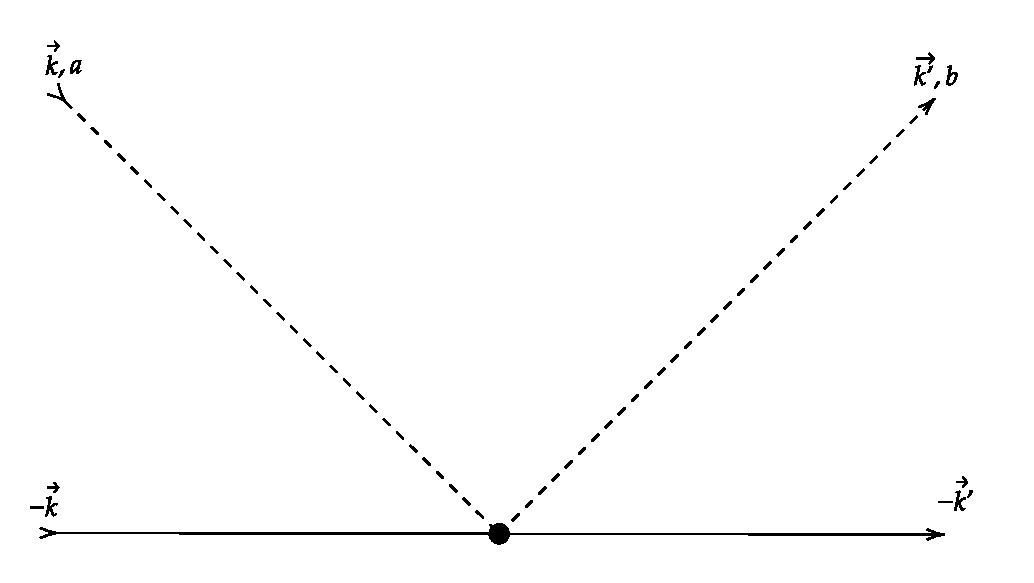
\includegraphics[scale=0.65]{1a.pdf}
\end{center}
\begin{align}
    \mm_{1,a}&= \frac{1}{4 F^2} v \cdot \left( \vec{k} +\vec{k}' \right) \varepsilon^{abc} \tau_c\\
             &= \frac{1}{4 F^2} (E_\pi+E_N)\varepsilon^{abc} \tau_c
\end{align}
We are in the CM frame, so $\vec{k}+\vec{k}'=0$, but $E_\pi\neq E_N$, but:
\begin{equation}
    \varepsilon^{abc} \tau_c= 0 \quad \text{for}\quad a=b   
\end{equation}
So this diagram is zero.
\newpage
%%%%%%%%%%%%%%%%%%%%%%%%%%%%%%%%%%%%%%%%%%%%%%%%%%%%%%%%%%%%%%%%%%%%%%%%%%%%%%%%%%%%%%%%%%%%%%%%%%%%%%%%%%%%%%%%%%%%%%
\subsection{1 Body B}

\begin{center}
    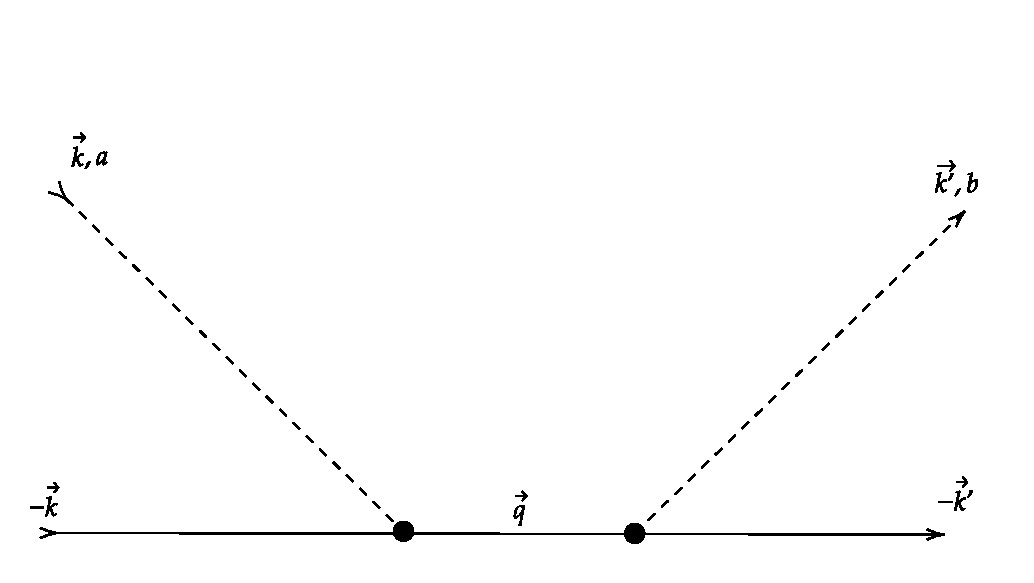
\includegraphics[scale=0.6]{1b.pdf}
\end{center}
\begin{align}
    \mm_{1,b}&=\left[-\frac{g_A}{F} S\cdot k \tau^a \right]\left( \frac{i}{v\cdot q + i \varepsilon} \right)
    \left[ \frac{g_A}{F} S\cdot k' \tau^b \right]\\
             &= -i\frac{g_A^2}{F^2}  \frac{\left( S\cdot k \right) \left( S\cdot k' \right)}{q_0 +i \varepsilon}  \tau^a \tau^b
\end{align}
$\vec{q}=0\implies q=(\sqrt{m_N^2+\vec{q}^{\,2}}, \vec{q}\,)=\mn$, and letting $S=(0,\frac{1}{2} \vec{\sigma})$ gives
\begin{align}
    \mm_{1,b}&= -i\frac{g_A^2}{F^2}  \frac{\left( S\cdot k \right) \left( S\cdot k' \right)}{\mn +i \varepsilon}  \tau^a \tau^b\\
             &= -i\frac{g_A^2}{4F^2}\; \frac{ \vec{\sigma}\cdot \vec{k}\; \vec{\sigma}\cdot \vec{k}\,' }{\mn +i \varepsilon}\; \tau^a \tau^b
\end{align}
\newpage
%%%%%%%%%%%%%%%%%%%%%%%%%%%%%%%%%%%%%%%%%%%%%%%%%%%%%%%%%%%%%%%%%%%%%%%%%%%%%%%%%%%%%%%%%%%%%%%%%%%%%%%%%%%%%%%%%%%%%%
\subsection{1 Body C}
\begin{center}
    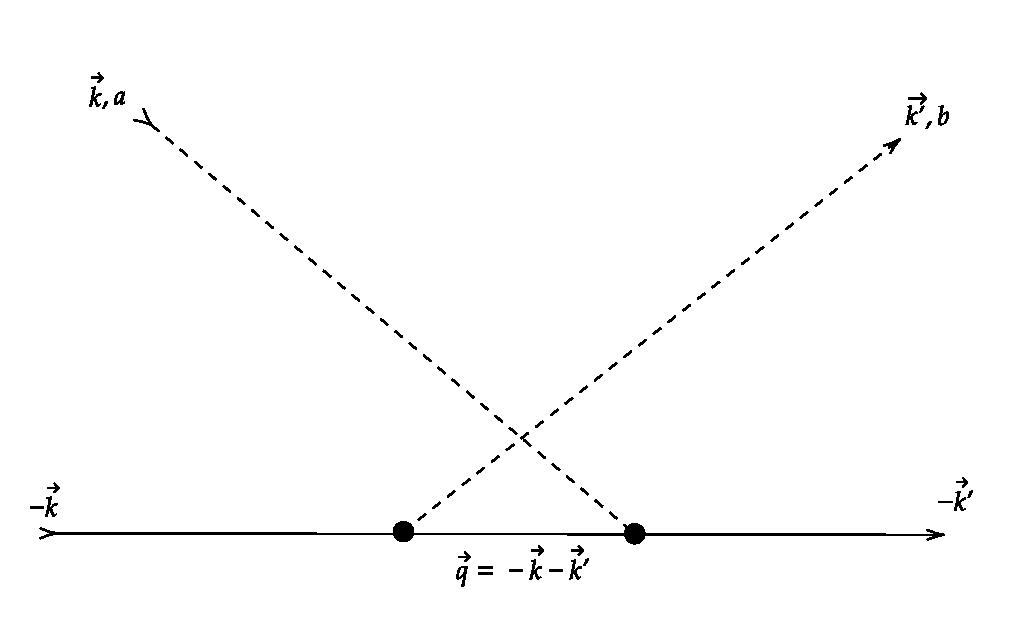
\includegraphics[scale=0.65]{1c.pdf}
\end{center}
This is the same as diagram B but with $\vec{q}=-\vec{k}-\vec{k}'$, so $q_0=\sqrt{\mn^2 + \vec{q}^{\:2}}$
\begin{align}
    \mm{1,c} &= -i\frac{g_A^2}{4F^2}\; \frac{ \vec{\sigma}\cdot \vec{k}\; \vec{\sigma}\cdot \vec{k}\,' }{q_0 +i \varepsilon}\; \tau^b \tau^a
\end{align}
\newpage
%%%%%%%%%%%%%%%%%%%%%%%%%%%%%%%%%%%%%%%%%%%%%%%%%%%%%%%%%%%%%%%%%%%%%%%%%%%%%%%%%%%%%%%%%%%%%%%%%%%%%%%%%%%%%%%%%%%%%%
\subsection{1 Body D}
Diagram 1 B, $\mo(p^3)$
\begin{center}
    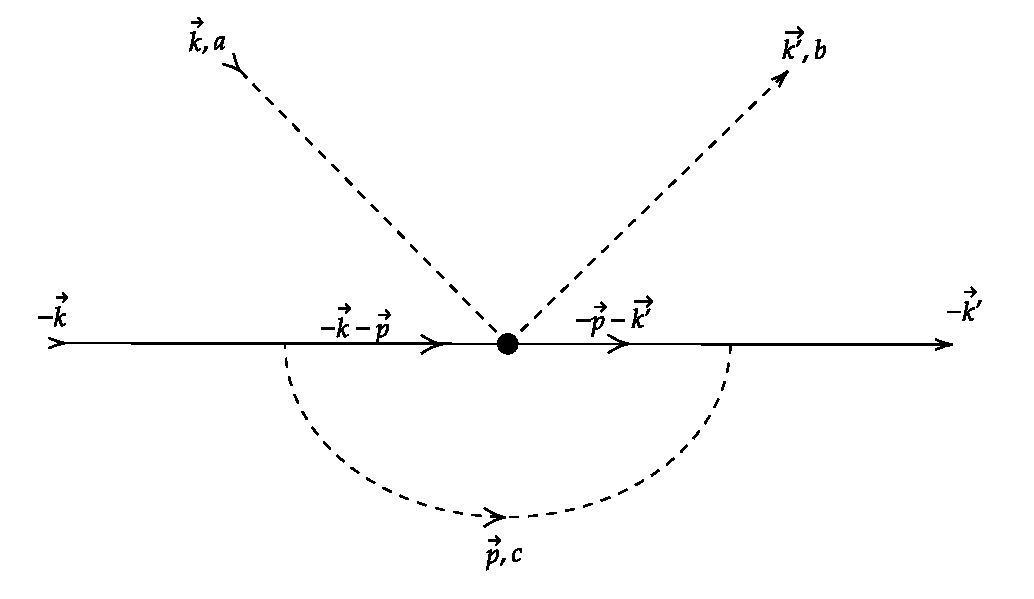
\includegraphics[scale=0.65]{1d.pdf}
\end{center}
Let $u=-k-p$ and $ u'=u+k-k'=-p-k'$
\begin{align}
    \mm_{1,d}&= \left[ \frac{g_A}{F} S \cdot p\, \tau^c  \right] i\left[\vec{u} \cdot \left( -\vec{k} - \vec{p} \right) +i \varepsilon  \right]^{-1} \left[\frac{1}{4 F^2} {v} \cdot \left( {k}+{k}' \right)\varepsilon^{abd} \tau^d \right]\nonumber \\
             &\times i \left[ \vec{u}^{\prime}\cdot \left( -\vec{p}-\vec{k}' \right) +i \varepsilon\right]^{-1}
             \left[ \frac{g_A}{F} {S}\cdot\left(-{p}\,\right)\tau^c\right]
             i[\vec{p}^{\,2} +i \varepsilon]^{-1}\\
             &=i\frac{g_A}{4 F^4} \; 
             \ddfrac{(S \cdot p\,)^2}{ \left( \vec{p}^{\,2} +i \varepsilon \right)  \left( \vec{u} \cdot \left(\vec{k} + \vec{p} \right) +i \varepsilon \right) \left( \vec{u}^{\prime}\cdot \left(\vec{p}+\vec{k}' \right) +i \varepsilon \right)}(E_\pi + E_\pi') \varepsilon^{abd} \tau^d\tau^c \tau_c  
\end{align}
Check this, did a lot of mental calculations
\newpage
%%%%%%%%%%%%%%%%%%%%%%%%%%%%%%%%%%%%%%%%%%%%%%%%%%%%%%%%%%%%%%%%%%%%%%%%%%%%%%%%%%%%%%%%%%%%%%%%%%%%%%%%%%%%%%%%%%%%%%
\subsection{1 Body E}
\begin{center}
    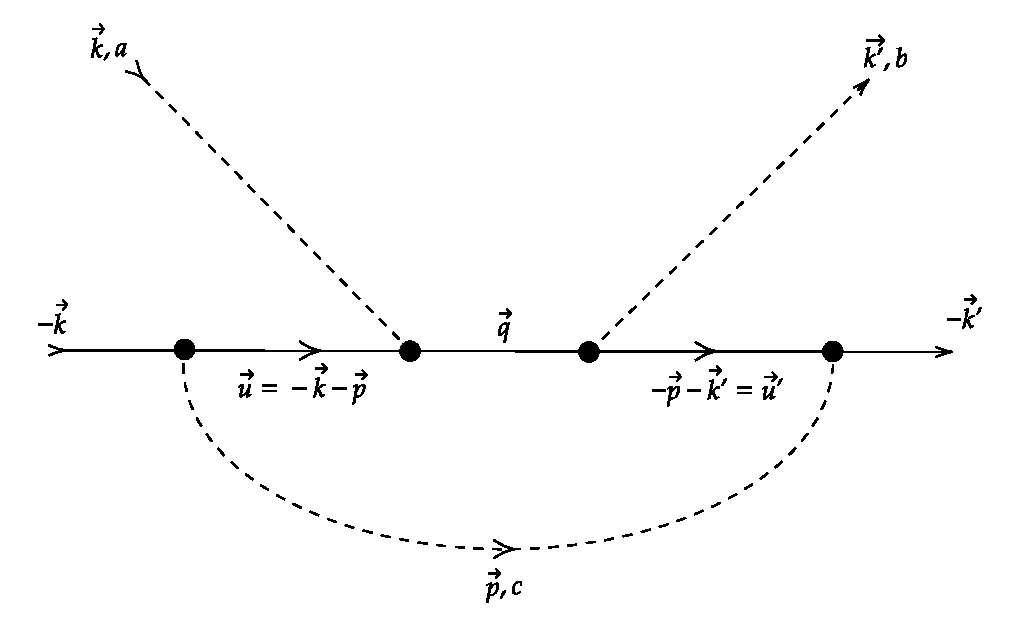
\includegraphics[scale=0.6]{1e.pdf}
\end{center}
\begin{align}
    \mm_{1,E}= &\left[ \frac{g_A}{F} S\cdot p \tau^c \right]
    \frac{i}{v\cdot (-k-p)+i \varepsilon }
    \left[-\frac{g_A}{F}\S \cdot k \tau^a \right]
    \left(\frac{1}{v\cdot q + i \varepsilon}\right)\nonumber\\
               &\times 
               \left(\frac{1}{p^2 - m_\pi^2 + i \varepsilon}\right)
               \left[\frac{g_A}{F}S \cdot k' \tau^b \right]
            \left(\frac{1}{v\cdot u' + i \varepsilon}\right)
            \left[-\frac{g_A}{F}S \cdot p \tau^c \right]
\end{align}
\newpage
%%%%%%%%%%%%%%%%%%%%%%%%%%%%%%%%%%%%%%%%%%%%%%%%%%%%%%%%%%%%%%%%%%%%%%%%%%%%%%%%%%%%%%%%%%%%%%%%%%%%%%%%%%%%%%%%%%%%%%
\subsection{1 Body F}
\begin{center}
    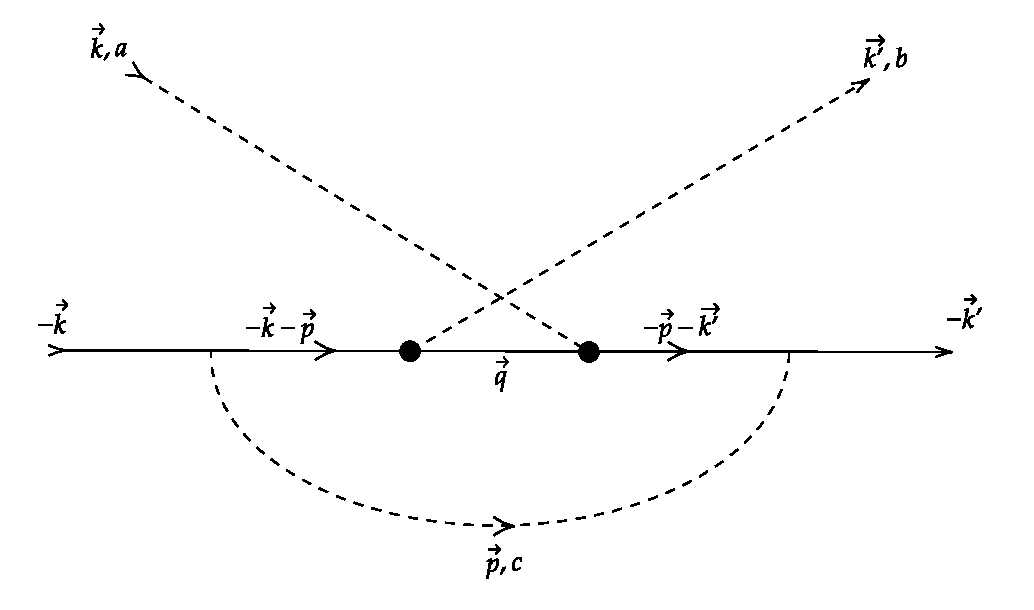
\includegraphics[scale=0.6]{1f.pdf}
\end{center}
\newpage
%%%%%%%%%%%%%%%%%%%%%%%%%%%%%%%%%%%%%%%%%%%%%%%%%%%%%%%%%%%%%%%%%%%%%%%%%%%%%%%%%%%%%%%%%%%%%%%%%%%%%%%%%%%%%%%%%%%%%%
\subsection{1 Body G}
Diagram 1 D, $\mo(p^4)$
\begin{center}
    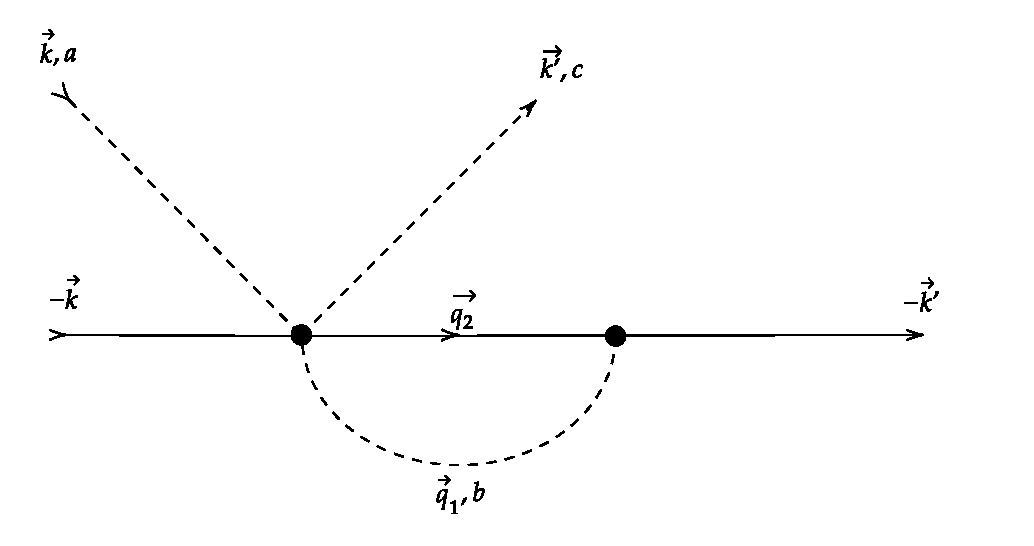
\includegraphics[scale=0.7]{1g.pdf}
\end{center}
Using BKM A.16
\begin{align}
    \mm_{1,d}&= \frac{g_A}{2F^3}  \left[ \tau^a \delta^{bc} S \cdot \left( q_1+k' \right)+ \tau^b \delta^{ac} S\cdot (-k+q_1) + \tau^c \delta^{ab} S\cdot(-k+q_1)\right]\nonumber\\
           &\quad\times i \left[ q_1^2 -m_{\pi}^2 +i \varepsilon \right]^{-1}
           i\left[v\cdot q_2 + i \varepsilon \right]^{-1}
           \left[ \frac{g_A}{F} S \cdot (-q_1) \tau^b\right]
\end{align}
\newpage
%%%%%%%%%%%%%%%%%%%%%%%%%%%%%%%%%%%%%%%%%%%%%%%%%%%%%%%%%%%%%%%%%%%%%%%%%%%%%%%%%%%%%%%%%%%%%%%%%%%%%%%%%%%%%%%%%%%%%%
\subsection{1 Body H}
Diagram 1 C, $\mo(p^4)$
\begin{center}
    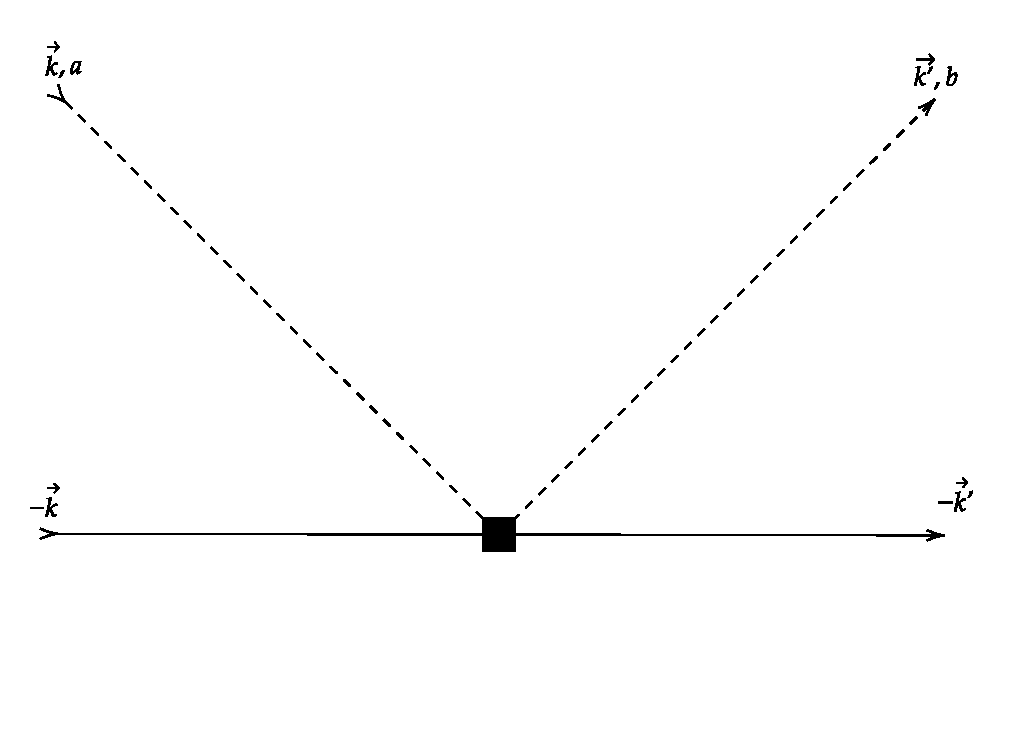
\includegraphics[scale=0.6]{1h.pdf}
\end{center}
Only Feynman rule is BKM review, A.29, but I'm not going to write it down here since its rather long, but here is a screenshot of the rule.
\begin{center}
    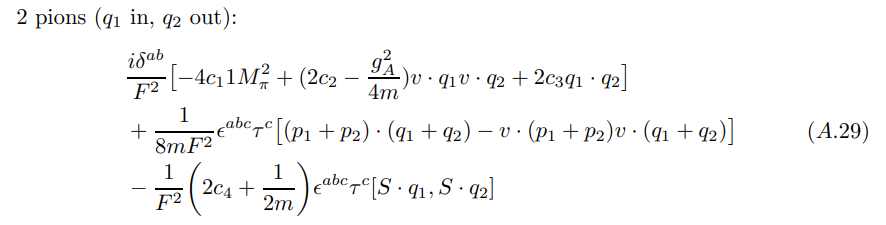
\includegraphics[scale=0.6]{A29-rule.png}
\end{center}
\newpage

%%%%%%%%%%%%%%%%%%%%%%%%%%%%%%%%%%%%%%%%%%%%%%%%%%%%%%%%%%%%%%%%%%%%%%%%%%%%%%%%%%%%%%%%%%%%%%%%%%%%%%%%%%%%%%%%%%%%%%
\subsection{1 Body I}
Diagram 1 C, $\mo(p^4)$
\begin{center}
    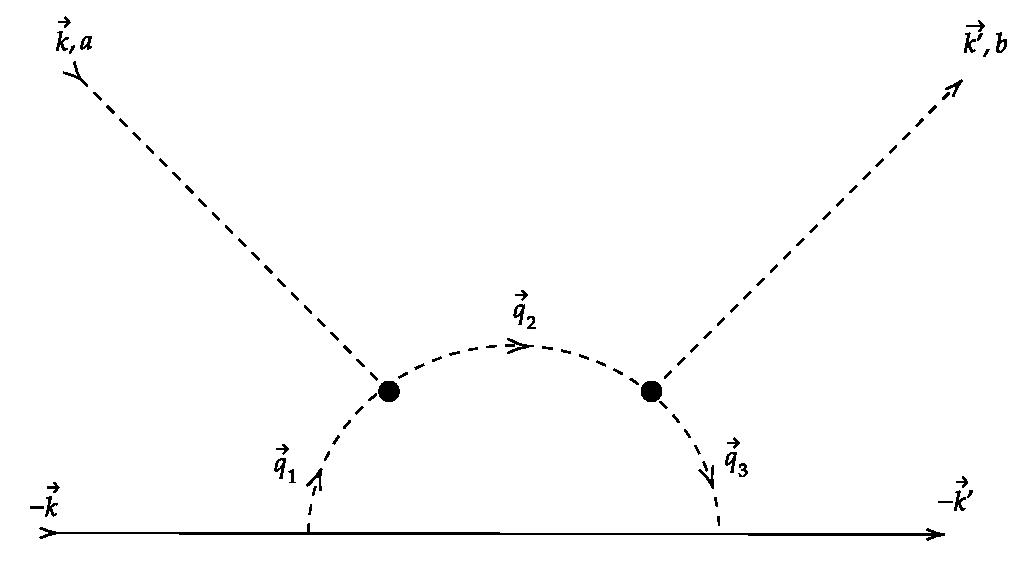
\includegraphics[scale=0.6]{1i.pdf}
\end{center}
This diagram is $0$, BKM A.3
\newpage
%%%%%%%%%%%%%%%%%%%%%%%%%%%%%%%%%%%%%%%%%%%%%%%%%%%%%%%%%%%%%%%%%%%%%%%%%%%%%%%%%%%%%%%%%%%%%%%%%%%%%%%%%%%%%%%%%%%%%%
%%%%%%%%%%%%%%%%%%%%%%%%%%%%%%%%%%%%%%%%%%%%%%%%%%%%%%%%%%%%%%%%%%%%%%%%%%%%%%%%%%%%%%%%%%%%%%%%%%%%%%%%%%%%%%%%%%%%%%
\section{2 Body Contributions}
Note that for the scattering length at least, there is a prefactor:
\begin{equation}
    \frac{1}{1+\mu} \equiv \alpha
\end{equation}
which comes from considerations other than the diagrams. Additionally, see BKM review equation 5.29:
\begin{equation}
    a_{ab}= \frac{1+ m_\pi/m_N}{1+m_\pi/Am_N} \sum_r a^{(r)}_{ab} + a^{\text{three-body}}_{ab}\label{bkmprefactor}
\end{equation}
Note for the BKM review "three-body" means two nucleons and an external probe, which is what we call two body.
In eq.(\ref{bkmprefactor}) $a,b$ are pion isospin indices, and $r$ (and later $s$ is used for this too) is for nucleon labeling. \\~\\

The BKM review states:
\begin{equation}
    (t_c^{(\pi)})_{ab}= -i \epsilon_{abc}\quad\text{is the pion isospin vector}
\end{equation}
But this only appears in the last diagram, and is specifically the pion isospin operator, not the nucleon isospin operator.
%%%%%%%%%%%%%%%%%%%%%%%%%%%%%%%%%%%%%%%%%%%%%%%%%%%%%%%%%%%%%%%%%%%%%%%%%%%%%%%%%%%%%%%%%%%%%%%%%%%%%%%%%%%%%%%%%%%%%%
\subsection{2 Body A}
\begin{center}
    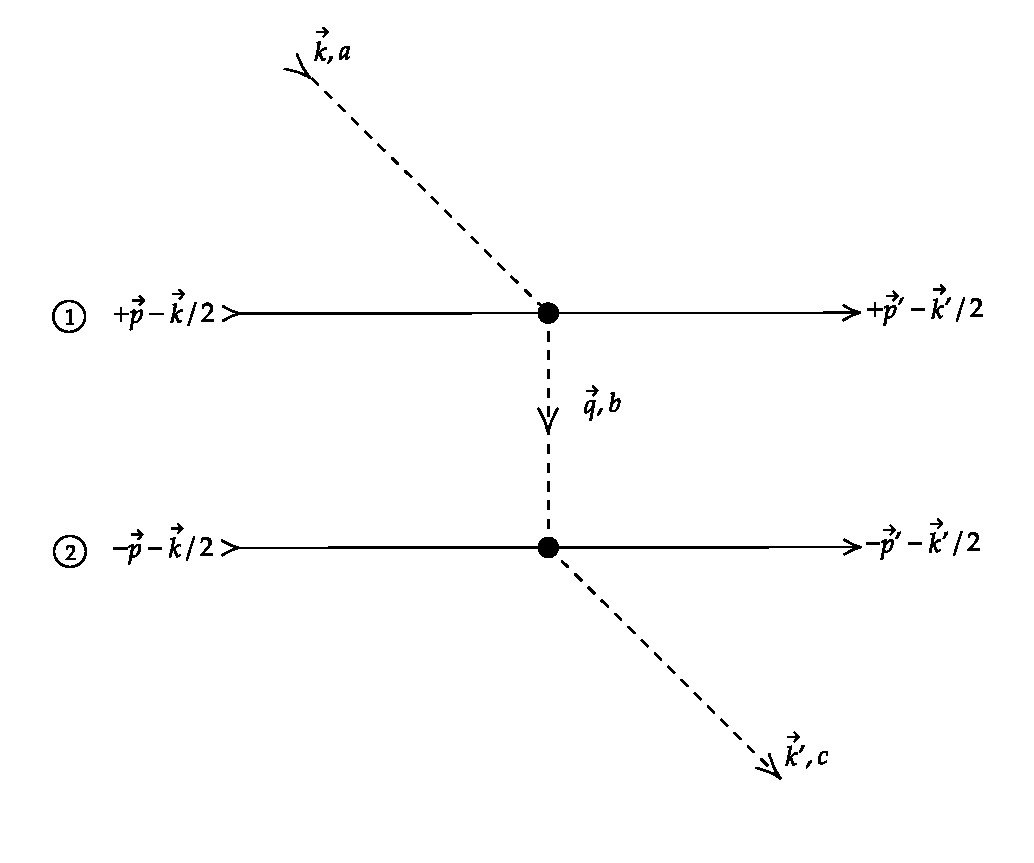
\includegraphics[scale=0.7]{2a.pdf}
\end{center}
Note $q=k/2+p$
\begin{align}
    \mm_{2,a}&=\alpha \left[\frac{1}{4 F^2} v \cdot \left( k+q \right) \varepsilon^{abd} \tau_1^d\right] i \left[ q^2-\mpi^2 + i \varepsilon \right]^{-1} \left[ \frac{1}{4 F^2} v^{\prime} \cdot \left( q + k' \right) \varepsilon^{bce} \tau_2^e \right]\\
             &=\alpha\left( \frac{1}{2 F}  \right)^4 
             \ddfrac{(E_\pi + q_0) (q_0+E_\pi')}{q^2 -m_\pi^2+i \varepsilon} \varepsilon^{abd}\varepsilon^{bce}\tau_1^d \tau_2^e
\end{align}
Where:
$\vec{q}=\vec{p} - \vec{p}\,' + \frac{1}{2} \left(\vec{k}+\vec{k}\,' \right)$, and $q_0=\sqrt{m_{\pi_0}^2 + \vec{q}\,^2}$
We now restrict ourselves to just the inelastic process, where $c=a$, then computing the matrix dependence gives:
\begin{align}
    \varepsilon^{abd} \varepsilon^{bae} \tau_1^d \tau_2^e
    &= -1 \left( \varepsilon^{bad} \varepsilon^{bae} \right)\tau_1^d \tau_2^e\\
    &= \left(\delta^{ae} \delta^{da}-\delta^{aa} \delta^{de} \right)\tau_1^d \tau_2^e\\
    &=(\delta^{ae} \delta^{da})\tau_1^d \tau_2^e-\tau_1^e \tau_{2e}\\
    &=\tau_1^a \tau_2^a-\tau_1^e \tau_{2e}
\end{align}
Here, the index $a$, is not being summed over. For example in the case of neutral pion pion scattering $a=3$ and this reduces to
\begin{equation}
    \tau_1^3 \tau_2^3-\vec{\tau}_1 \cdot \vec{\tau}_2
\end{equation}
So the diagram contribution is then:
\begin{align}
    \mm_{2,a} &= \left( \frac{1}{2 F}  \right)^4 
    \ddfrac{(E_\pi + q_0) (q_0+E_\pi')}{q^2 - m_\pi^2+i \varepsilon} \left( \tau_1^a \tau_2^a-\vec{\tau}_1 \cdot \vec{\tau}_2 \right)
\end{align}
Or in the threshold case: 

\begin{align}
    \mm_{2,a} &= \left( \frac{1}{2 F}  \right)^4 
    \ddfrac{m_\pi^2}{\vec{q}^{\;2}+i \varepsilon} \left( \tau_1^a \tau_2^a-\vec{\tau}_1 \cdot \vec{\tau}_2 \right)
\end{align}
For this diagram, at threshold, Beane gets the result:
\begin{equation}
    \frac{M_\pi^2}{32\pi^4 F_\pi^4 (1+ \mu/2)} \frac{1}{\vec{q}\;^2} 
\end{equation}
And Weinberg for the threshold case writes the result as (eq 5):
\begin{align}
    \frac{M_\pi^2}{32\pi^4 F_\pi^4 (1+ \mu/2)}\sum_{r<s} \frac{1}{\vec{q}_{rs}\;^2}  \left( 2 \vec{\tau}^{(r)} \cdot \vec{\tau}^{(s)} \delta_{ab}-t_a^{(r)} t_b^{(s)} - t_a^{(s)} t_b^{(r)} \right)
\end{align}
Taking $a=b$ the above reduces to:
\begin{align}
    \frac{M_\pi^2}{16\pi^4 F_\pi^4 (1+ \mu/2)}\sum_{r<s} \frac{1}{\vec{q}_{rs}\;^2}  \left( \vec{\tau}^{(r)} \cdot \vec{\tau}^{(s)}-t_a^{(r)} t_a^{(s)}\right)
\end{align}
\note{What do we do about this sum?}
%%%%%%%%%%%%%%%%%%%%%%%%%%%%%%%%%%%%%%%%%%%%%%%%%%%%%%%%%%%%%%%%%%%%%%%%%%%%%%%%%%%%%%%%%%%%%%%%%%%%%%%%%%%%%%%%%%%%%%
\subsection{2 Body B}
Diagram b (at threshold) according to Weinberg is:
\begin{align}
    - \frac{g_A^2 \delta_{ab}}{32 \pi^4 F_\pi^4 (1+\mu)} \vec{\tau}_1 \cdot \vec{\tau}_2
    \ddfrac{\vec{q}\cdot \vec{\sigma}_1 \vec{q} \cdot \vec{\sigma}_2}{\vec{q}^{\,2} + m_\pi^2} 
\end{align}
and the Beane paper gives the result for diagram $b$ and $c$ together as:
\begin{equation}
    - \frac{g_A^2 m_\pi^2}{128 \pi^4 F_\pi^4 (1+\mu)} 
    \ddfrac{\vec{q}\cdot \vec{\sigma}_1 \vec{q} \cdot \vec{\sigma}_2}{(\vec{q}^{\,2} + m_\pi^2)^2} 
\end{equation}
Using BKM A.16 - check indicies.
\begin{center}
    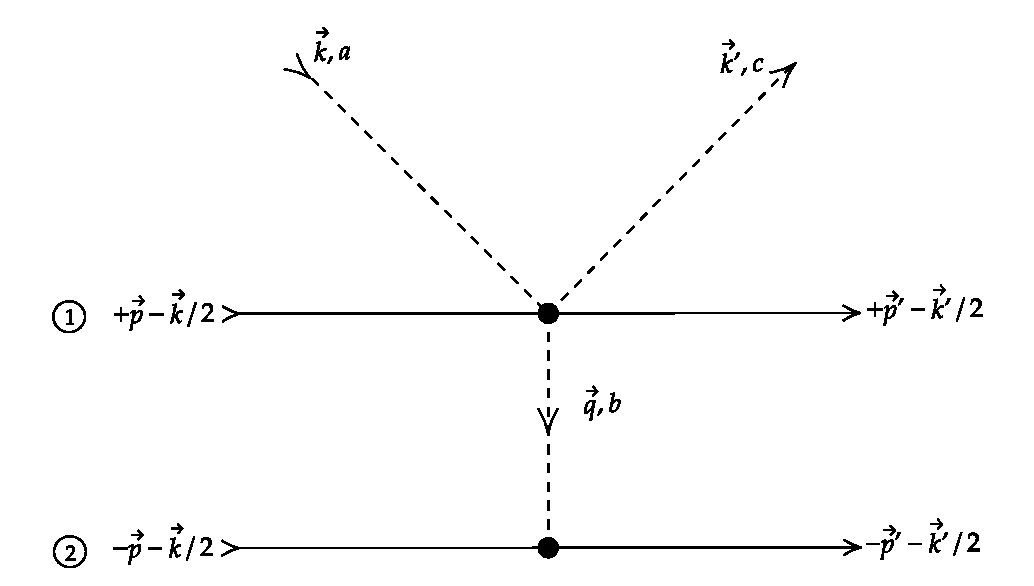
\includegraphics[scale=0.9]{2b.pdf}
\end{center}
\begin{align}
\mm_{2,b}&=\frac{g_A}{2F^3} \left[ \tau^a \delta^{bc} S_1 \cdot(q+k') + \tau^b \delta^{ac} S_1 \cdot(k'-k)+ \tau^c \delta^{ab} S_1 \cdot \left( q-k \right)\right]\nonumber\\
             &\times i \left[ q^2-\mpi^2 +i \varepsilon \right]^{-1} \left[ \frac{g_A}{F} S_2\cdot(-q) \tau^b \right]\\
             % &=-i\frac{g_A^2}{8 F^4} \frac{1}{\vec{q}^{\,2} + i \varepsilon} 
             % \vec{\sigma}_1 \cdot\left[ \tau^a \delta^{bc} (\vec{q}+\vec{k}') + \tau^b \delta^{ac} (\vec{k}\,'-\vec{k})+ \tau^c \delta^{ab} \left( \vec{q}-\vec{k} \right)\right] \vec{\sigma}_2\cdot \vec{q}\, \tau^b
\end{align}
The Feynman rule for 3 pions (all qs out) is just:
\begin{equation}
    \frac{g_A}{2F^3}\left[ \tau^a \delta^{bc} S_1 \cdot(q_2+q_3) + \tau^b \delta^{ac} S_1 \cdot(q_1+q_3)+ \tau^c \delta^{ab} S_1 \cdot \left(q_1+q_2\right)\right]
\end{equation}
% Substitute:
% \begin{align}
%     &S_1^\mu= \frac{1}{2} \left( I, \vec{\sigma} \right)\\%= \frac{1}{2} \vec{\sigma}^\mu\\
%     \text{But note}\quad& S_{1,\mu}= \frac{1}{2} \left( I, -\vec{\sigma} \right)
% \end{align}
And we have:
\begin{equation}
    \vec{q}_1=-\vec{k}\quad \vec{q}_2=\vec{q} \quad \vec{q}_3=\vec{k}'
\end{equation}
The last $\tau$ should be operating on the second nucleon, and the other $\tau$ operators are supposed to be on nucleon 1. Additionally, the index $b$, must be summed over, whereas $a$ and $c$ are external observables (pion isospin). The index $b$ is the only one that is summed over.
\begin{align}
\mm_{2,b}&=-i\frac{g_A^2}{8F^4}\frac{1}{q^{\;2}- m_\pi^2 + i \varepsilon} \sum_{b=1}^3 S_1 \cdot \left[ \tau_1^a \delta^{bc} (q_2+q_3) + \tau_1^b \delta^{ac} (q_1+q_3)+ \tau_1^c \delta^{ab} \left(q_1+q_2\right)\right] S_2 \cdot q_2 \tau^b_2\\
             % &=-i\frac{g_A^2}{8F^4}\frac{1}{q^{\;2}- m_\pi^2 + i \varepsilon} S_1 \cdot \left[ \tau_1^a \delta^{ba} (q_2+q_3) + \tau_1^b \delta^{aa} (q_1+q_3)+ \tau_1^a \delta^{ab} \left(q_1+q_2\right)\right] S_2 \cdot q \tau^b_2\label{Correct}
               &=-i\frac{g_A^2}{8F^4}\frac{1}{q^{\;2}- m_\pi^2 + i \varepsilon} \sum_{b=1}^3 S_1 \cdot \left[ \tau_1^a\tau_2^b \delta^{bc} (q_2+q_3) + \tau_1^b \tau_2^b\delta^{ac} (q_1+q_3)+ \tau_2^b\tau_1^c \delta^{ab} \left(q_1+q_2\right)\right] S_2 \cdot q_2\label{Correct}\\
               &=-i\frac{g_A^2}{8F^4}\frac{1}{q^{\;2}- m_\pi^2 + i \varepsilon} \sum_{b=1}^3 S_1 \cdot \left[ \tau_1^a\tau_2^b \delta^{bc} (q_2+q_3) + \vec{\tau}_1 \cdot \vec{\tau}_2 \delta^{ac}(q_1+q_3)+ \tau_2^b\tau_1^a \delta^{ab} \left(q_1+q_2\right)\right] S_2 \cdot q_2\\
    &=-i\frac{g_A^2}{8F^4}\frac{1}{q^{\;2}- m_\pi^2 + i \varepsilon} S_1 \cdot \left[ \tau_1^a\tau_2^c (q_2+q_3) +3\vec{\tau}_1 \cdot \vec{\tau}_2 (q_1+q_3)\delta^{ac}+ \tau_2^a\tau_1^a \left(q_1+q_2\right)\right] S_2 \cdot q_2\\
    &=-i\frac{g_A^2}{8F^4}\frac{1}{q^{\;2}- m_\pi^2 + i \varepsilon} S_1 \cdot \left[ \tau_1^a\tau_2^c (q_1+2q_2+q_3) +3\vec{\tau}_1 \cdot \vec{\tau}_2 \delta^{ac}(q_1+q_3)\right] S_2 \cdot q_2
\end{align}
Now taking $a=c$:
\begin{align}
 \mm_{2,b}&=-i\frac{g_A^2}{8F^4}\frac{1}{q^{\;2}- m_\pi^2 + i \varepsilon} S_1 \cdot \left[ \tau_1^a\tau_2^a (q_1+2q_2+q_3) +3\vec{\tau}_1 \cdot \vec{\tau}_2 (q_1+q_3)\right] S_2 \cdot q_2
\end{align}
Note that $q_2$ is the propagator momentum and is therefore off shell.
Now taking the limit of the threshold case, $q_1=q_3=(m_\pi, \vec{0})$ and $q_2=(0,\vec{q})$, and the non-relativistic limit of $S=(0,\vec{\sigma})$:
\begin{align}
    \mm_{2,b}&=i\frac{g_A^2}{16F^4}\frac{\tau_1^a\tau_2^a}{\vec{q}^{\;2}+ m_\pi^2 - i \varepsilon}\left(\vec{\sigma}_1 \cdot \vec{q} \right)\left(\vec{\sigma}_2 \cdot \vec{q}\right)
\end{align}
Which is really close to the Weinberg result, except for a factor of $\left[2\pi^4 \left( 1+\mu \right)\right]^{-1}]$ and the constant $a$ should be a sum. Note that the factors of $\pi$ are fixed if we use $F \to \pi F_\pi$.
Also, I wonder if the sum over $a$ comes from allowing any pion to propagate instead of just the neutral pion.

% \subsubsection{Analysis for $S=(0,\frac{1}{2} \vec{\sigma}) $}
% This section and the following section can be ignored. The discussion of the definition of $S$ occurs in the first section.\\~\\
% For the following, note that:
% \begin{equation}
%     S_0 q_0 - \vec{S} \cdot \vec{q} = S \cdot q
% \end{equation}
% In order to compare my result to the Beane and Weinberg result consider the threshold case: $\vec{k}=\vec{k}'=0$, and we don't know if they use $S=(0, \frac{1}{2} \vec{\sigma})$, or $S=(\mathbbm{1}, \frac{1}{2} \vec{\sigma})$, so we start with just the first one.
% Now use $\vec{q}_1=-\vec{k}\quad \vec{q}_2=\vec{q} \quad \vec{q}_3=\vec{k}'$, and drop the energy component on each of the vectors
% \begin{align}
%     \mm_{2,b}&=-i\frac{g_A^2}{8F^4}\frac{1}{q^{\;2}- m_\pi^2 + i \varepsilon} \frac{1}{4} \sigma_1 \cdot \left[ \tau_1^a\tau_2^a (q_1+2q_2+q_3) +3\vec{\tau}_1 \cdot \vec{\tau}_2 (q_1+q_3)\right] \sigma_2 \cdot q\\
%              &=-i\frac{g_A^2}{8F^4}\frac{1}{q^{\;2}- m_\pi^2 + i \varepsilon} \frac{1}{4} \vec{\sigma}_1 \cdot \left[ \tau_1^a\tau_2^a (-\vec{k}+2\vec{q}+\vec{k}') +3\vec{\tau}_1 \cdot \vec{\tau}_2 (-\vec{k}+\vec{k}')\right] \vec{\sigma}_2 \cdot \vec{q}
% \end{align}
% Now taking the threshold case:
% \begin{align}
%     \mm_{2,b} &=-i\frac{g_A^2}{16F^4}\frac{\tau_1^a\tau_2^a}{q^{\;2}- m_\pi^2 + i \varepsilon} \vec \sigma_1 \cdot \vec{q}\;\vec\sigma_2 \cdot \vec{q}\label{base}
% \end{align}



% \subsubsection{Analysis for $S=(\mathbbm{1},\frac{1}{2} \vec{\sigma}) $}
% \begin{align}
%     \mm_{2,b}&=-i\frac{g_A^2}{8F^4}\frac{1}{q^{\;2}- m_\pi^2 + i \varepsilon} S_1 \cdot \left[ \tau_1^a\tau_2^a (q_1+2q_2+q_3) + \vec{\tau}_1 \cdot \vec{\tau}_2 (q_1+q_3)\right] S_2 \cdot q\\
% \end{align}
% Looking at this by parts, but in the threshold case:
% \begin{align}
%      &S_1 \cdot \left[ \tau_1^a\tau_2^a (q_1+2q_2+q_3) +3\vec{\tau}_1 \cdot \vec{\tau}_2 (q_1+q_3)\right] S_2 \cdot q\\
%      &S_1 \cdot \left[ \tau_1^a\tau_2^a (q_1+2q_2+q_3) +3\vec{\tau}_1 \cdot \vec{\tau}_2 (q_1+q_3)\right] S_2 \cdot q\\
%     =& \tau_1^a \tau_2^b \left(2 m_\pi +2 q_0 - \vec{\sigma}_1 \cdot \vec{q}\right)+6m_\pi\vec{\tau}_1 \cdot \vec{\tau}_2\left( q_0 - \frac{1}{2} \vec{\sigma}_2 \cdot \vec{q}\right)
% \end{align}
% Consider just $S \to (\mathbbm{1}, \vec{0})$
% \begin{align}
%      &S_1 \cdot \left[ \tau_1^a\tau_2^a (q_1+2q_2+q_3) +3\vec{\tau}_1 \cdot \vec{\tau}_2 (q_1+q_3)\right] S_2 \cdot q\\
%      =& \left( \tau_1^a\tau_2^a (m_\pi+2 q_0 +m_\pi) +3\vec{\tau}_1 \cdot \vec{\tau}_2 (m_\pi+m_\pi)\right) q_0\\
%      =& \left( \tau_1^a\tau_2^a (2 m_\pi+2 q_0) +6 m_\pi\vec{\tau}_1 \cdot \vec{\tau}_2 \right) q_0\\
% \end{align}
% This is the "difference" between the two results, so I think we can conclude $S= \left( 0, \frac{1}{2} \vec{\sigma}  \right) $


\subsubsection{The Propagator}
Weinberg writes the structure of the propagator as:
$(\vec{q}\sq +m_\pi^2)^{-1} $
Whereas Beane writes it as:
$(\vec{q}\sq +m_\pi^2)^{-2}$
But the "starting" propagator as defined in BKM A.1 is 
$i \delta^{ab} \left( q^2 -m_\pi^2 + i \varepsilon \right)^{-1}$, where $q$ is the four momentum.
Now we can write the propagator as :
\begin{align}
    \left[ q^2-m_\pi^2 \right]^{-1}&= \left[ E^2 -\vec{q}\sq -m_\pi^2 \right]^{-1}\\
                                   &= \frac{-1}{\vec{q}\sq +m_\pi^2} \left[ 1- \left( \ddfrac{E^2}{\vec{q}\sq +
                                   m_\pi^2}  \right) \right]^{-1}\\
                                   &= \frac{-1}{\vec{q}\sq +m_\pi^2} \left[ 1 + \frac{E^2}{\vec{q}\sq +m_\pi^2}+
                                   \left(\frac{E^2}{\vec{q}\sq +m_\pi^2}\right)^2 +... \right]
\end{align}
Where $E=\sqrt{m_\pi^2 + \vec{q}\sq}$. So now taking the threshold case $m_\pi\gg\vec{q}\sq$

\begin{align}
    \left[ q^2-m_\pi^2 \right]^{-1}&\approx \frac{-1}{\vec{q}\sq + m_\pi^2} \left[ 1+ \frac{m^2_\pi}{\vec{q}\sq +m_\pi^2} +... \right]\\
                 &\approx \frac{-1}{\vec{q}\sq + m_\pi^2} \left[ 1+ \frac{m^2_\pi}{\vec{q}\sq +m_\pi^2} +... \right]
\end{align}
But I'm confused why Weinberg bothered with this, it's not that much more complicated to just program the initial propagator. Maybe its to avoid numerical zeros.
\begin{align}
    \mm_{2,b} &=-i\frac{g_A^2}{16F^4}\tau_1^a\tau_2^a\vec \sigma_1 \cdot \vec{q}\;\vec\sigma_2 \cdot \vec{q} 
    \left[\frac{-1}{\vec{q}\sq +m_\pi^2} + \mathcal{O}(q_0^2) \right]
\end{align}
So then:
\begin{align}
    \mm_{2,b} &=i\frac{g_A^2}{16F^4}\tau_1^a\tau_2^a \;\frac{\vec{\sigma}_1 \cdot \vec{q}\;\vec\sigma_2 \cdot \vec{q} }{\vec{q}\sq +m_\pi^2}
\end{align}
But this is still different than the Weinberg result by a factor of $2$ and the isospin dependence.
%%%%%%%%%%%%%%%%%%%%%%%%%%%%%%%%%%%%%%%%%%%%%%%%%%%%%%%%%%%%%%%%%%%%%%%%%%%%%%%%%%%%%%%%%%%%%%%%%%%%%%%%%%%%%%%%%%%%%%
%%%%%%%%%%%%%%%%%%%%%%%%%%%%%%%%%%%%%%%%%%%%%%%%%%%%%%%%%%%%%%%%%%%%%%%%%%%%%%%%%%%%%%%%%%%%%%%%%%%%%%%%%%%%%%%%%%%%%%
%%%%%%%%%%%%%%%%%%%%%%%%%%%%%%%%%%%%%%%%%%%%%%%%%%%%%%%%%%%%%%%%%%%%%%%%%%%%%%%%%%%%%%%%%%%%%%%%%%%%%%%%%%%%%%%%%%%%%%
%%%%%%%%%%%%%%%%%%%%%%%%%%%%%%%%%%%%%%%%%%%%%%%%%%%%%%%%%%%%%%%%%%%%%%%%%%%%%%%%%%%%%%%%%%%%%%%%%%%%%%%%%%%%%%%%%%%%%%
%%%%%%%%%%%%%%%%%%%%%%%%%%%%%%%%%%%%%%%%%%%%%%%%%%%%%%%%%%%%%%%%%%%%%%%%%%%%%%%%%%%%%%%%%%%%%%%%%%%%%%%%%%%%%%%%%%%%%%
\subsection{2 Body C}
\begin{center}
    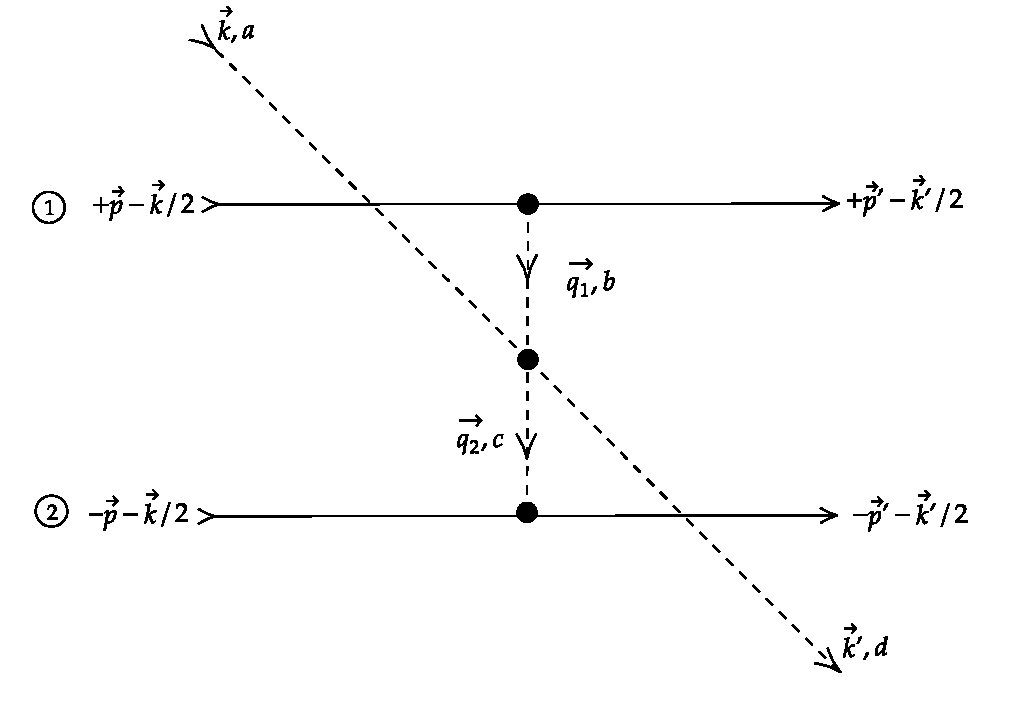
\includegraphics[scale=0.8]{2c.pdf}
\end{center}
With:
\begin{align}
    \vec{q}_1&= \vec{p}-\vec{p}\,' + \frac{1}{2} ( \vec{k}'-\vec{k})\\
    \vec{q}_2&= \vec{p}-\vec{p}\,' + \frac{1}{2} ( \vec{k}'+\vec{k})
\end{align}
Using BKM A.10, with all $q$'s in
\begin{equation}
    O^{abcd}=\frac{i}{F^2} \Bigg\{
         \delta^{ab}\delta^{cd} \left[ (q_1+q_2)^2 - \mpi^2 \right]+
    \delta^{ac}\delta^{bd} \left[ \left( q_1+q_3\right)^2 -m_\pi^2 \right]
             +\delta^{ad}\delta^{bc} \left[ \left(q_1+q_4 \right)^2 - m_\pi^2 \right]
     \Bigg\}
\end{equation}
From BKM (left hand side), to our labels, (right hand side)
\begin{align}
    &\text{Matrix indices}\;a,b,c,d\;\text{ remain the same}\\
    &\vec q_1 \to \vec{q}_1\quad \text{index}\;b \\
    &\vec q_2 \to \vec{k}\quad \text{index}\;a \\
    &\vec q_3 \to -\vec{q}_2\quad \text{index}\;c \\
    &\vec q_4 \to -\vec{k}'\quad \text{index}\;d
\end{align}
\begin{align}
    \mm_{2,c}&=\frac{g}{F} S_1 \cdot q_1 \tau_1^b  i \left[ q_1 -m_\pi^2 + i \varepsilon \right]^{-1}
     O^{abcd}
    \frac{g}{F}   S_2 \cdot(-q_2) \tau_2^c
    i \left[ q_2^2 -m_\pi^2 + i \varepsilon \right]^{-1}\\
    &=\frac{g}{F} S_1 \cdot q_1 \tau_1^b  i \left[ q_1 -m_\pi^2 + i \varepsilon \right]^{-1}
     \frac{i}{F^2} 
     O^{abcd}
    \frac{g}{F}   S_2 \cdot(-q_2) \tau_2^c
    i \left[ q_2^2 -m_\pi^2 + i \varepsilon \right]^{-1}\\
    &=-i \frac{g^2}{F^4} S_1 \cdot q_1\; S_2 \cdot(-q_2) O^{abcd}
    \frac{\tau_1^b \tau_2^c}{
    (q_1^2 -m_\pi^2 + i \varepsilon)
    (q_2^2-m_\pi^2 + i \varepsilon)
    }
\end{align}
I'm sure this is correct, but there is some weird stuff going on with the energy flow.
In particular $q_1^2 =-\vec{q}_1\sq$, but $q_2^2=E_2^2 - \vec{q}_2\sq$.
Also note that $O^{abcd}$ has no isospin dependence, so we can commute $\tau$ with it. This gives:
\begin{align}
    \mm_{2,c}&=i \frac{g^2}{F^4} S_1 \cdot q_1\; S_2 \cdot(-q_2) 
    \frac{\tau_1^b \tau_2^c}{
        (\vec{q}_1\sq +m_\pi^2 + i \varepsilon)
        (E_2^2-\vec{q}_2\sq-m_\pi^2 + i \varepsilon)
    }
    O^{abcd}
\end{align}
Where $E_2$ is the 
%%%%%%%%%%%%%%%%%%%%%%%%%%%%%%%%%%%%%%%%%%%%%%%%%%%%%%%%%%%%%%%%%%%%%%%%%%%%%%%%%%%%%%%%%%%%%%%%%%%%%%%%%%%%%%%%%%%%%%
%%%%%%%%%%%%%%%%%%%%%%%%%%%%%%%%%%%%%%%%%%%%%%%%%%%%%%%%%%%%%%%%%%%%%%%%%%%%%%%%%%%%%%%%%%%%%%%%%%%%%%%%%%%%%%%%%%%%%%
%%%%%%%%%%%%%%%%%%%%%%%%%%%%%%%%%%%%%%%%%%%%%%%%%%%%%%%%%%%%%%%%%%%%%%%%%%%%%%%%%%%%%%%%%%%%%%%%%%%%%%%%%%%%%%%%%%%%%%
%%%%%%%%%%%%%%%%%%%%%%%%%%%%%%%%%%%%%%%%%%%%%%%%%%%%%%%%%%%%%%%%%%%%%%%%%%%%%%%%%%%%%%%%%%%%%%%%%%%%%%%%%%%%%%%%%%%%%%
%%%%%%%%%%%%%%%%%%%%%%%%%%%%%%%%%%%%%%%%%%%%%%%%%%%%%%%%%%%%%%%%%%%%%%%%%%%%%%%%%%%%%%%%%%%%%%%%%%%%%%%%%%%%%%%%%%%%%%
\subsection{2 Body D}
\begin{center}
    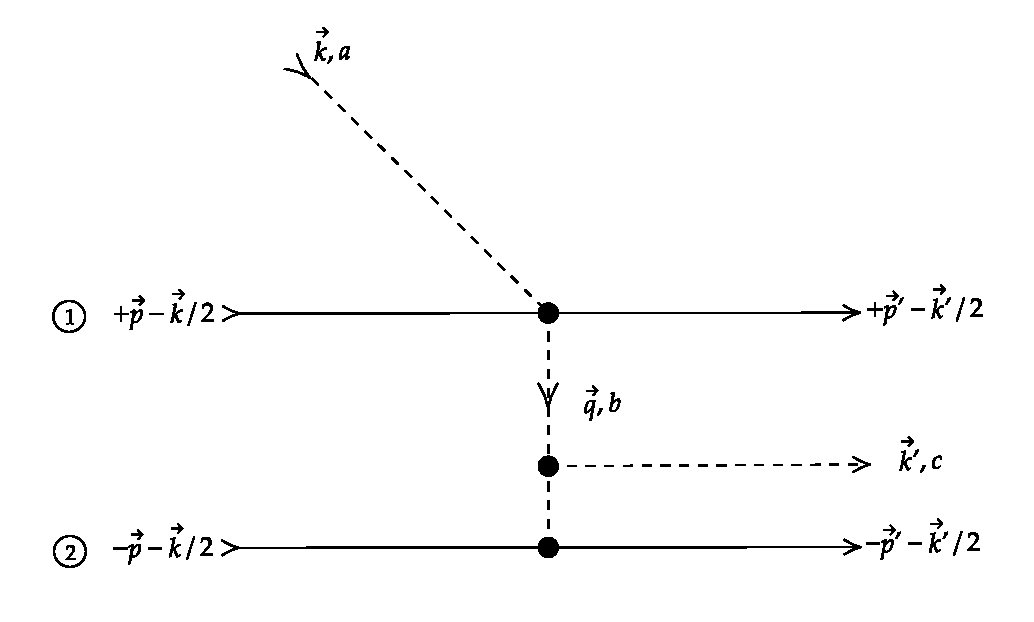
\includegraphics[scale=0.6]{2d.pdf}
\end{center}
\section{Two Body contributions to the scattering length}
As stated in the BKM review pg 115-116 the two body contributions to the scattering length from the first six diagrams is:
\begin{align}
    a_{ab}&= \frac{M_\pi^2}{32 \pi^4 F_\pi^4\left(1+M_\pi / m_d\right)} \sum_{r<s}\left\langle\frac{1}{\vec{q}_{r s}^2}\left(2 \vec{\tau}^{(r)} \cdot \vec{\tau}^{(s)} \delta_{a b}-\tau_a^{(r)} \tau_b^{(s)}-\tau_a^{(s)} \tau_b^{(r)}\right)\right\rangle\\
          & -\frac{g_A^2 \delta_{a b}}{32 \pi^4 F_\pi^4\left(1+M_\pi / m_d\right)} \sum_{r<s}\left\langle\vec{\tau}^{(r)} \cdot \vec{\tau}^{(s)} \frac{\vec{q}_{r s} \cdot \vec{\sigma}^{(r)} \vec{q}_{r s} \cdot \vec{\sigma}^{(s)}}{\vec{q}_{r s}^2+M_\pi^2}\right\rangle \\
          &+\frac{g_A^2}{32 \pi^4 F_\pi^4\left(1+M_\pi / m_d\right)} \sum_{r<s}\left\langle\frac{\left[\vec{q}_{r s}^2 \vec{\tau}^{(r)} \cdot \vec{\tau}^{(s)} \delta_{a b}+M_\pi^2\left(\tau_a^{(r)} \tau_b^{(s)}+\tau_a^{(s)} \tau_b^{(r)}\right) \vec{q}_{r s} \cdot \vec{\sigma}^{(r)} \vec{q}_{r s} \cdot \vec{\sigma}^{(s)}\right.}{\left(\vec{q}_{r s}^2+M_\pi^2\right)^2}\right\rangle \\
          &+\frac{g_A^2 M_\pi}{132 \pi^4 F_\pi^4\left(1+M_\pi / m_d\right)} \sum_{r<s}\left\langle\left(\vec{\tau}^{(r)}+\vec{\tau}^{(s)}\right) \cdot\left(\vec{\tau}^{(\pi)}\right)_{a b} \frac{\vec{q}_{r s} \cdot \vec{\sigma}^{(r)} \vec{q}_{r s} \cdot \vec{\sigma}^{(s)}}{\left(\vec{q}_{r s}^2+M_\pi^2\right)^{3 / 2}}\right\rangle\label{lasteq}
\end{align}
Note that $\left(\vec{\tau}^{(\pi)}\right)_{ab}=-i\varepsilon_{abc}$, where $\varepsilon$ is the Levi-Civita Tensor, with $a,b$ being the pion isospin indices.
In this analysis we consider only elastic scattering so $a=b \implies\left(\vec{\tau}^{(\pi)}\right)_{aa}=-i\varepsilon_{aac}=\vec{0}$ so eq.(\ref{lasteq}) drops out.\\~\\
In order to implement the above terms in our code I will write them in a manner more useful for us.
The BKM review uses the notation $(r), (s)$ to indicate nucleon number but we simply use $1,2$, and the integration over the other nucleons is accounted for elsewhere.
Additionally we can simplify using $a=b$.
Additionally we seek to write the isospin dependence in terms of the actual quantum numbers $t_{12}, m_{12}$ etc.
Now let:
\begin{equation}
    \beta= \frac{1}{32 \pi^4 F_\pi^4 (1+M_\pi/M_{\text{nucl}})} 
\end{equation}
Simplifying we have:
\begin{align}
    a&= 2 \beta M_\pi^2\left\langle\frac{1}{\vec{q}^2}\left(\vec{\tau}_1 \cdot \vec{\tau}_2 -\tau^a_{1} \tau^a_{2}\right)\right\rangle\nonumber\\
     &-\beta g_A^2 \left\langle\vec{\tau}_{1} \cdot \vec{\tau}_{2} \frac{\vec{q} \cdot \vec{\sigma}_{1} \vec{q} \cdot \vec{\sigma}_{2}}{\vec{q}\sq+M_\pi^2}\right\rangle \\
     &+\beta g_A^2\left\langle\frac{\left[\vec{q}\sq \vec{\tau}_1 \cdot \vec{\tau}_2 +2 M_\pi^2\;\left(\tau^a_{1} \tau^a_{2}\right)\; ]\vec{q} \cdot \vec{\sigma}_{1} \vec{q}\cdot \vec{\sigma}_{2}\right.}{\left(\vec{q}\sq+M_\pi^2\right)^2}\right\rangle\nonumber
\end{align}
Recall:
\begin{align}
\br{t'_{12} m_{12}^{t'}\;s'_{12} m'_{12}}\vec{\tau}_1\cdot \vec{\tau}_2 \kt{t_{12} m_{12}^t\;s_{12} m_{12}}= \delta_{s'\ot s\ot} \delta_{m'\ot m\ot} \delta_{t'\ot t\ot}\delta_{m^{t'}\ot m^{t}\ot}\bigg[2 t_{12} (t_{12} +1) -3\bigg]
\end{align}
And from an internal communication with Harald Griesshammer 
\begin{equation}
\br{t'_{12} m_{12}^{t'}}\vec{\tau}_1\cdot \vec{\tau}_2 - \tau_1^a \tau_2^a \kt{t_{12} m_{12}^t}=
\left\{
\begin{array}{ll}
    -2 (-1)^{t\ot}&\quad\text{if}\quad t'\ot=t\ot\quad\text{and}\quad m^{t'}\ot =m^{t}\ot=0\\
    0&\quad\text{otherwise}
\end{array}
\right.
\end{equation}
Note the above holds for $t=0,1$ and $|m^t\ot|\leq t$.
Equivalently we can write this as:
\begin{equation}
\br{t'_{12} m_{12}^{t'}}\vec{\tau}_1\cdot \vec{\tau}_2 - \tau_1^a \tau_2^a \kt{t_{12} m_{12}^t}=
\delta_{t'\ot,t\ot} \delta_{m^{t'}\ot, m^t\ot} \delta_{m^t\ot,0}(-2)(-1)^{t\ot}
\end{equation}
So then, using $M_J, M'_J$ as a shorthand for all the quantum numbers:
\begin{align}
    \br{M_J'}\tau_1^a \tau_2^a \kt{M_J}&= \br{M_J'}\vec{\tau}_1 \cdot \vec{\tau}_2-\big[\vec{\tau}_1 \cdot \vec{\tau}_2 - \tau_1^a \tau_2^a \big] \kt{M_J}\\
                                       &=\delta_{s\ot,s\ot'}\delta_{m\ot,m\ot'}\delta_{m_{12}^{t'}{m_{12}^{t}}} \delta_{\tot,\totp} \Bigg[ \big( 2 t_{12} \left( \tot+1 \right) -3\big) - \delta_{m_{12}^t ,0} \left( -2 \right) (-1)^{t_{12}}\Bigg]
\end{align}
Now we only care about $t_{12}=0,1$ and $|m^t\ot|\leq t\ot$ so we can just evaluate the above for those cases.
\begin{equation}
    \big( 2 t_{12} \left( \tot+1 \right) -3\big) - \delta_{m_{12}^t ,0} \left( -2 \right) (-1)^{t_{12}}= (-1)^{m\ot^t+1}\quad
    \text{for}\quad t_{12}=0,1,\;\;|m^t\ot|\leq t\ot
\end{equation}
So:
\begin{align}
    \br{M_J'}\tau_1^a \tau_2^a \kt{M_J}&= \delta_{s\ot,s\ot'}\delta_{m\ot,m\ot'}\delta_{m_{12}^{t'}{m_{12}^{t}}} \delta_{\tot,\totp} (-1)^{m^t\ot+1}
\end{align}
The spin dependence $\vec{q}\cdot \vec{\sigma}_1 \vec{q}\cdot \vec{\sigma}_2$ is taken care of in our code already so I will not include it here. So now making these substitutions for the isospin dependence we have:
\begin{align}
    a=\delta_{t'_{12},t_{12}} \delta_{m^{t'}\ot, m^t\ot}&\Bigg[ -4 \beta M_\pi^2 
        \frac{1}{\vec{q}\sq}(-1)^{t\ot}\delta_{s\ot,s\ot'}\delta_{m_{12},m\ot'}\delta_{m^t_{12},0}\nonumber\\
     &-\beta g_A^2 \Big[ 2 t\ot (t\ot+1)-3 \Big] \frac{\vec{q} \cdot \vec{\sigma}_{1} \vec{q} \cdot
     \vec{\sigma}_{2}}{\vec{q}\sq+M_\pi^2}\nonumber\\
          &+\beta g_A^2\frac{\vec{q}\sq \Big[2 t\ot \left( t\ot+1)-3 \right) \Big]\vec{q} \cdot \vec{\sigma}_{1} \vec{q}\cdot \vec{\sigma}_{2}}{\left(\vec{q}\sq+M_\pi^2\right)^2}\nonumber\\
          &-2\beta g_A^2 M_\pi^2\frac{\;(-1)^{m^t_{12}}\; \vec{q} \cdot \vec{\sigma}_{1} \vec{q}\cdot \vec{\sigma}_{2}}{\left(\vec{q}\sq+M_\pi^2\right)^2}\Bigg]
\end{align}
We still need to account for the $+(1\leftrightarrow2)$ to the extent that it is not already accounted for in the subroutines.
\end{document}
